\documentclass[10pt]{memoir}
\setstocksize{220mm}{155mm} 	        
\settrimmedsize{220mm}{155mm}{*}	
\settypeblocksize{170mm}{116mm}{*}	
\setlrmargins{18mm}{*}{*}
\setulmargins{*}{*}{1.2}
%\setlength{\headheight}{5pt}%
\checkandfixthelayout[lines]
\linespread{1.16}
\flushbottom

%%% Hyphenation settings
\usepackage[htt]{hyphenat}
\hyphenation{he-lio-trope opos-sum}
\tracingparagraphs=1
%Hyphenation in Devanāgarī of the edition still missing? Probably this needs to be modified in babel-iast package? 

%%% babel
\usepackage[english]{babel}
\usepackage{babel-iast/babel-iast}

\babelfont[iast]{rm}[Renderer=Harfbuzz, Scale=1.3]{AdishilaSan}%AdishilaSan}
\babelfont[english]{rm}{Adobe Text Pro}

%%% more functionality
\PassOptionsToPackage{hyphens}{url}
\usepackage{hyperref}
\usepackage{pdflscape}
\usepackage{cleveref}
\usepackage{url}
\usepackage{cleveref}
\usepackage{microtype}
\usepackage{lineno}

%\usepackage{bigfoot}
%%% more functions
\usepackage[dvipsnames]{xcolor}
%\usepackage[para,perpage]{footmisc}

%%%für den Counter von Kapiteln und Sätzen! 
\newcommand{\uproman}[1]{\uppercase\expandafter{\romannumeral#1}}
\newcommand{\lowroman}[1]{\romannumeral#1\relax}

\makeindex
\newfontfamily\sanskritfont[Script=Devanagari,Mapping=RomDev,Scale=1.1]{Sanskrit2003}
\usepackage{pifont,fourier-orns,lettrine,psvectorian,paralist,enumitem,pdfpages,wrapfig,tabulary,lettrine,longtable}
\setlist[enumerate]{itemsep=0mm}
\usepackage[autostyle]{csquotes}
\usepackage[defaultlines=2,all]{nowidow}
\usepackage{ellipsis,adforn,booktabs,longtable,url,tikz}
\lineskiplimit=-3pt          

\makechapterstyle{IeT}{%
  \chapterstyle{default}
  \renewcommand*{\printchapternonum}{\centering}
  \renewcommand*{\clearforchapter}{\cleartorecto} 
  \aliaspagestyle{chapter}{empty}}
\chapterstyle{IeT}
\setsecnumdepth{none}  \openright  \nouppercaseheads
\settocdepth{subsubsection}

%%%% test better pagebreaks
%\def\fussy{%
%  \emergencystretch\z@
%  \tolerance 200%
%  \hfuzz .1\p@
%  \vfuzz\hfuzz}

%\interfootnotelinepenalty=10000\relax

%\usepackage[maxfloats=256]{morefloats}

%\maxdeadcycles=500

%raggedbottomsectiontrue
%%\checkandfixthelayout


%%%%%%%  biblatex
%\newcommand{\noun}[1]{\textsc{#1}}    %  philosophy-verbose
\usepackage[backend=biber, sorting=nyt, style=verbose]{biblatex} %%%%ORIGINAL TiE
\renewcommand*{\mkbibnamefamily}[1]{\textsc{#1}}


\DeclareFieldFormat{url}{%
  \mkbibacro{URL}\addcolon\space
  \href{#1}{\nolinkurl{\thefield{urlraw}}}}

\DeclareFieldFormat{citeurl}{%
  \href{#1}{\nolinkurl{\thefield{urlraw}}}} 


\DeclareFieldFormat{postnote}{#1}
\renewcommand{\postnotedelim}{, }
\addbibresource{bindu.bib}

%%% ekdosis
\usepackage[teiexport=tidy,parnotes=true]{ekdosis}% =tidy cleans up HTML and XML documents by fixing markup errors and upgrading legacy code to modern standards. parnotes=footnotes below or above critical apparatus

\SetLineation{lineation=page, modulo} %lineation=page sets thenumbering to start afresh at the top of each page. =modulo makes every fifth line numbered. {lineation=page} makes every line numbered! 

\renewcommand{\linenumberfont}{\selectlanguage{english}\footnotesize} %sets language of lines to English

\SetTEIxmlExport{autopar=false} %autopar=falseinstructs ekdosis to ignore blank lines in the.tex sourcefile as markers for paragraph boundaries. As a result, each paragraph of the edition must be found within an environment associated with the xml <p> element

\SetHooks{
  lemmastyle=\bfseries,
  %refnumstyle=\selectlanguage{english}\bfseries,
  refnumstyle=\selectlanguage{english}\color{blue}\bfseries,
  appheight=0.8\textheight,
}

\newif\ifinapparatus
\DeclareApparatus{source}[
%bhook=\inapparatustrue,
lang=english,
notelang=english,
% bhook=\selectlanguage{english},
bhook=\selectlanguage{english}\textbf{Sources:},%
%maxentries=4, 
%ehook=.]
%sep={] },
%nosep,
]

\newif\ifinapparatus
\DeclareApparatus{testium}[
%bhook=\inapparatustrue,
lang=english,
notelang=english,
% bhook=\selectlanguage{english},
bhook=\selectlanguage{english}\textbf{Testimonia:},
%maxentries=4, 
%ehook=.]
%nosep, 
]

% Declare \ifinapparatus and set \inapparatustrue at the beginning of
% the apparatus criticus block. Also set the language.  
\newif\ifinapparatus
  \DeclareApparatus{default}[
  %bhook=\inapparatustrue, 
  lang=english,
  %maxentries=33,
  %bhook=\selectlanguage{english},
  sep = {] },
  delim=\hskip 0.75em,
  rule=\rule{0.7in}{0.4pt},
]

\newif\ifinapparatus
\DeclareApparatus{philcomm}[
%bhook=\inapparatustrue,
lang=english,
notelang=english,
bhook=\selectlanguage{english}\textbf{Philological Commentary:},
%bhook=\selectlanguage{english},
sep={: },
]

\ekdsetup{
showpagebreaks,
spbmk = \textcolor{blue}{spb},
hpbmk = \textcolor{red}{hpb}
}

%\usepackage{fnpos}
%\makeFNmid
%\makeFNbottom
\usepackage[bottom]{footmisc}
%%%%%%%%%%%%%%%%%%%%%%%%%%%
\makeatletter
\def\blfootnote{\gdef\@thefnmark{}\@footnotetext}
\makeatother
%%%%%%%%%%%%%%%%%%%%%%%%%


% Macros and Definitions for the Print of Sigla
\def\acpc#1#2#3{{#1}\rlap{\textrm{\textsuperscript{#3}}}\textsubscript{\textrm{#2}}\space}
\def\sigl#1#2{{{#1}}\textsubscript{\textrm{#2}}}
\def\None{{\sigl{N}{1}}} \def\Noneac{\acpc{N}{1}{ac}\,} \def\Nonepc{\acpc{N}{1}{pc}\,}
\def\Ntwo{{\sigl{N}{2}}} \def\Noneac{\acpc{N}{2}{ac}\,} \def\Nonepc{\acpc{N}{2}{pc}\,}
\def\Done{{\sigl{D}{1}}} \def\Doneac{\acpc{D}{1}{ac}\,} \def\Donepc{\acpc{D}{1}{pc}\,}
\def\Dtwo{{\sigl{D}{2}}} \def\Dtwoac{\acpc{D}{2}{ac}\,} \def\Dtwopc{\acpc{D}{2}{pc}\,}
\def\Uone{{\sigl{U}{1}}} \def\Uoneac{\acpc{U}{1}{ac}\,} \def\Uonepc{\acpc{U}{1}{pc}\,}                 
\def\Utwo{{\sigl{U}{2}}} \def\Utwoac{\acpc{U}{2}{ac}\,} \def\Utwopc{\acpc{U}{2}{pc}\,}

%%%%%%%%%%%%%% Tattvabinduyoga - List of Witnesses   %%%%%%%%%%%%%%%%%%%
\DeclareWitness{ceteri}{\selectlanguage{english}cett.}{ceteri}[]   
\DeclareWitness{E}{\selectlanguage{english}E}{Printed Edition}[]    
\DeclareWitness{P}{\selectlanguage{english}P}{Pune BORI 664}[]  
\DeclareWitness{B}{\selectlanguage{english}B}{Bodleian 485}[]       
\DeclareWitness{N1}{\selectlanguage{english}N\textsubscript{1}}{NGMPP 38/31}[]
\DeclareWitness{N2}{\selectlanguage{english}N\textsubscript{2}}{NGMPP B 38/35}[]
\DeclareWitness{L}{\selectlanguage{english}L}{LALCHAND 5876}[]  
\DeclareWitness{D}{\selectlanguage{english}D}{IGNCA 30019}[] 
%\DeclareWitness{D2}{\selectlanguage{english}D\textsubscript{2}}{IGNCA 30020}[]  
\DeclareWitness{U1}{\selectlanguage{english}U\textsubscript{1}}{SORI 1574}[] 
\DeclareWitness{U2}{\selectlanguage{english}U\textsubscript{2}}{SORI 6082}[]
%%%%%%%%%%%%%% Tattvabinduyoga - Groups of Witnesses   %%%%%%%%%%%%%%%%%%%
\DeclareWitness{X}{\selectlanguage{english}\alpha}{Alpha Group: D,N1,N2,U1}[]
\DeclareWitness{Y}{\selectlanguage{english}\beta}{Beta Group: B,E,L,P,U2}[]
%%%%%%%%%%%%% Testimonia
\DeclareWitness{Ysv}{\selectlanguage{english}Ysv}{Yogasvarodaya}[] %%%add infos!  

%%%%%%%%%%%%%%%%%%%%%%%%%%%%%%%%%%%%%%%%%%%
% Macro for Editing Abbrevs.
\def\om{\textrm{\footnotesize \textit{om.}\ }} %prints om. for omitted in apparatus
\def\korr{\textrm{\footnotesize \textit{em.}\ }} %prints em. for emended in apparatus
\def\conj{\textrm{\footnotesize \textit{conj.}\ }} %prints conj. for conjectured in apparatus

% \supplied{text} EDITORIAL ADDITION -> Within \lem oder \rdg
% \surplus{text} EDITORIAL DELETION -> Within \lem oder \rdg
% \sic{text} CRUX
% \gap{text} LACUNAE -> [reason=??, unit=??, quantity=??, extent=??]


%%%%%%%%%%%%%%%%%%%%%%%%%%%%%%%%%%%%%%%%%%% All macros of this list can be used in 
% Macro for Editing Abbrevs.
\def\eyeskip{\textrm{{ab.\,oc. }}}
\def\aberratio{\textrm{{ab.\,oc. }}}
\def\ad{\textrm{{ad}}}
\def\add{\textrm{{add.\ }}}
\def\ann{\textrm{{ann.\ }}}
\def\ante{\textrm{{ante }}} 
\def\post{\textrm{{post }}}
%\def\ceteri{cett.\,}                   
\def\codd{\textrm{{codd.\ }}}

\def\coni{\textrm{{coni.\ }}}
\def\contin{\textrm{{contin.\ }}}
\def\corr{\textrm{{corr.\ }}}
\def\del{\textrm{{del.\ }}}
\def\dub{\textrm{{ dub.\ }}}

\def\expl{\textrm{{explic.\ }}} 
\def\explica t{\textrm{{explic.\ }}}
\def\fol{\textrm{{fol.\ }}}
\def\foll{\textrm{{foll.\ }}}
\def\gloss{\textrm{{glossa ad }}}
\def\ins{\textrm{{ins.\ }}}      
\def\inseruit{\textrm{{ins.\ }}} 
\def\im{{\kern-.7pt\lower-1ex\hbox{\textrm{\tiny{\emph{i.m.}}}\kern0pt}}} %\textrm{\scriptsize{i.m.\ }}}      
\def\inmargine{{\kern-.7pt\lower-.7ex\hbox{\textrm{\tiny{\emph{i.m.}}}\kern0pt}}}%\textrm{\scriptsize{i.m.\ }}}      
\def\intextu{{\kern-.7pt\lower-.95ex\hbox{\textrm{\tiny{\emph{i.t.}}}\kern0pt}}}%\textrm{\scriptsize{i.t.\ }}}           
\def\indist{\textrm{{indis.\ }}}  
\def\indis{\textrm{{indis.\ }}}
\def\iteravit{\textrm{{iter.\ }}} 
\def\iter{\textrm{{iter.\ }}}
\def\lectio{\textrm{{lect.\ }}}   
\def\lec{\textrm{{lect.\ }}}
\def\leginequit{\textrm{{l.n. }}} 
\def\legn{\textrm{{l.n. }}}
\def\illeg{\textrm{{l.n. }}}

\def\primman{\textrm{{pr.m.}}}
\def\prob{\textrm{{prob.}}}
\def\rep{\textrm{{repetitio }}}
\def\secundamanu{\textrm{\scriptsize{s.m.}}}            \def\secm{{\kern-.6pt\lower-.91ex\hbox{\textrm{\tiny{\emph{s.m.}}}\kern0pt}}}%   \textrm{\scriptsize{s.m.}}}
\def\sequentia{\textrm{{seq.\,inv.\ }}}  
\def\seqinv{\textrm{{seq.\,inv.\ }}}
\def\order{\textrm{{seq.\,inv.\ }}}
\def\supralineam{{\kern-.7pt\lower-.91ex\hbox{\textrm{\tiny{\emph{s.l.}}}\kern0pt}}} %\textrm{\scriptsize{s.l.}}}
\def\interlineam{{\kern-.7pt\lower-.91ex\hbox{\textrm{\tiny{\emph{s.l.}}}\kern0pt}}}   %\textrm{\scriptsize{s.l.}}}
\def\vl{\textrm{v.l.}}   \def\varlec{\textrm{v.l.}} \def\varialectio{\textrm{v.l.}}
\def\vide{\textrm{{cf.\ }}}
\def\cf{\textrm{{cf.\ }}} 
\def\videtur{\textrm{{vid.\,ut}}}
\def\crux{\textup{[\ldots]} }
\def\cruxx{\textup{[\ldots]}}
\def\unm{\textit{unm.}}
%%%%%%%%%%%%%%%%%%%%%%%%%%%%%%%%%%%%

% List of Scholars
\DeclareScholar{ego}{ego}[
forename=Nils Jacob,
surname=Liersch]

% Persons:14\DeclareScholar{ego}{ego}[15forename=Robert,16surname=Alessi]17% Useful shorthands:18\DeclareShorthand{codd}{codd.}{V,I,R,H}19\DeclareShorthand{edd}{edd.}{Lit,Erm,Sm}20\DeclareShorthand{egoscr}{\emph{scripsi}}{ego}

%Useful shorthands:
%\DeclareShorthand{codd}{codd.}{V,I,R,H}
%\DeclareShorthand{edd}{edd.}{Lit,Erm,Sm}
\DeclareShorthand{egoscr}{em.}{ego}
\DeclareShorthand{egoscrconj}{conj.}{ego}
\DeclareShorthand{egomute}{\unskip}{ego}

\usepackage{xparse}

\NewDocumentEnvironment{tlg}{O{}O{}}{\setlength{\leftskip}{0pt}\vspace{-1ex}\begin{quotation}}{\hfill #1\ \vspace{-1ex}\end{quotation}\vspace{-1ex}} %verse environment
%\NewDocumentEnvironment{tlg}{O{}O{}}{\begin{verse}}{॥#1\hskip-4pt ॥\\ \end{verse}}
\NewDocumentCommand{\tl}{m}{{\selectlanguage{iast} #1}}

\NewDocumentCommand{\extra}{m}{{\textcolor{gray}{#1}}} %command for additions to U2
\NewDocumentCommand{\crazy}{m}{{\textcolor{red}{#1}}} %totally corrupted passage
\NewDocumentCommand{\coro}{m}{{\textcolor{violet}{#1}}} %colour for sentence counter! 

\NewDocumentEnvironment{prose}{O{}}{\begin{otherlanguage}{iast}}{\end{otherlanguage}}
% \NewDocumentEnvironment{padd}{O{}}{\begin{otherlanguage}{iast}}{\end{otherlanguage}}
\NewDocumentEnvironment{tlate}{O{}}
%\NewDocumentEnvironment{tadd}{O{}}

%Define two commands: \skp ("sanskrit plus"), to be ignored by TeX in
%the edition text, but processed in the TEI output. Conversely, \skm
%("sanskrit minus") is to be processed in the edition text, but
%ignored if found in the apparatus criticus and in the TEI output:

\NewDocumentCommand{\skp}{m}{}
\TeXtoTEIPat{\skp {#1}}{#1}

%\NewDocumentCommand{\skpp}{m}{}
%\TeXtoTEIPat{\skpp {#1}}{#1}

\NewDocumentCommand{\skm}{m}{\unless\ifinapparatus#1-\fi}
\TeXtoTEIPat{\skm {#1}}{}

% \NewDocumentCommand{\dd}{}{/\hskip-4pt/}
\NewDocumentCommand{\dd}{}{\mbox{/\hskip-4pt/}}
\TeXtoTEIPat{\dd {}}{//}


%%% modify environments and commands
%%% TEI mapping
\TeXtoTEIPat{\begin {tlg}}{<lg>} %lg=(Group of verse (s)) contains one or more verses or lines of verse that together form a formal unit (e.g. stanza, chorus).
\TeXtoTEIPat{\end {tlg}}{</lg>}

\TeXtoTEIPat{\begin {prose}}{<p>}
\TeXtoTEIPat{\end {prose}}{</p>}

\TeXtoTEIPat{\begin {tlate}}{<p>}
\TeXtoTEIPat{\end {tlate}}{</p>}

\TeXtoTEIPat{\\}{}
\TeXtoTEIPat{\linebreak}{<br/>}
\TeXtoTEIPat{\noindent}{}
%\TeXtoTEI{tl}{l}
\TeXtoTEI{emph}{hi}
\TeXtoTEI{bigskip}{}
\TeXtoTEI{None}{N1}
\TeXtoTEI{Ntwo}{N2}
\TeXtoTEI{Done}{D1}
\TeXtoTEI{Dtwo}{D2}
\TeXtoTEI{Uone}{U1}
\TeXtoTEI{Utwo}{U2}
%\TeXtoTEIPat{/}{ |}
%\TeXtoTEI{//}{ ||}
\TeXtoTEIPat{\korr}{em. }
\TeXtoTEIPat{\conj}{conj.}
\TeXtoTEIPat{\om}{om.}
\TeXtoTEIPat{english}{}
\TeXtoTEIPat{\hskip}{}
\TeXtoTEIPat{\hskip-4pt}{}
\TeXtoTEIPat{\hskip-2pt}{}
\TeXtoTEIPat{-}{ }
\TeXtoTEIPat{4pt}{}
\TeXtoTEIPat{2pt}{}
\TeXtoTEIPat{\textcolor {#1}{#2}}{<hi rend="#1">#2</hi>} 

% Nullify \selectlanguage in TEI as it has been used in
% \DeclareWitness but should be ignored in TEI.
\TeXtoTEI{selectlanguage}{}



\FormatDiv{1}{\begin{center}\Large}{\end{center}}
\FormatDiv{2}{\begin{center}\small}{\end{center}}
\FormatDiv{3}{\bfseries}{.}
\title{Yogatattvabindu of Rāmacandra\\ A Critical Edition and Annotated Translation}
\date{\today}

\parindent=15pt
\begin{document}

% Zitiermöglichkeiten:
%\footcite[See][p.\,1]{goldstein01:_tibet_englis_diction_moder_tibet}
%\footnote{\cite{goldstein01:_tibet_englis_diction_moder_tibet}.}

\frontmatter
\thispagestyle{empty}
\begin{center}
  {\Large \emph{The Yogatattvabindu}}\\[3mm]
\end{center}



\newpage

\

\thispagestyle{empty}



\normalsize


\newpage


\begin{center}
\thispagestyle{empty}

\

\vskip 2mm

\begin{otherlanguage}{iast}
\LARGE \sanskritfont{Yogatattvabindu}
\end{otherlanguage}

\vskip .4cm

\Huge Yogatattvabindu \\[7mm]
\Large Critical Edition\\
with annotated Translation


\large

\vspace{3cm}

Von

Nils Jacob Liersch
\small
\vfill

\vfill

Indica et Tibetica Verlag \\ % $\cdot$ 
Marburg 2024

\vskip 6mm

\end{center}

\newpage
\newpage \ \thispagestyle{empty}
\small  \

\noindent

\
\vfill


\small
\noindent \textbf{Bibliographische Information Der Deutschen Bibliothek}

\noindent
Die Deutsche Bibliothek verzeichnet diese Publikation in der Deutschen Nationalbibliographie;
detaillierte bibliographische Informationen sind im Internet über http://dnb.ddb.de abrufbar.

\noindent
\textbf{Bibliographic information published by Die Deutschen Bibliothek}

\noindent
Die Deutsche Bibliothek lists this publication in the Deutsche Nationalbibliographie; detailed
bibliographic data is available in the Internet at http://dnb.ddb.de.  


\vskip 1cm

\noindent
\copyright\ Indica et Tibetica Verlag, Marburg 2024

\medskip

\noindent
Alle Rechte vorbehalten / All rights reserved

\medskip

\noindent
Ohne ausdrückliche Genehmigung des Verlages ist es nicht gestattet, das Werk oder einzelne Teile
daraus nachzudrucken, zu vervielfältigen oder auf Datenträger zu speichern.

\smallskip

\noindent
Apart from any fair dealing for the purpose of private study, research, criticism or review, no
part of this book may be reproduced or translated in any form, by print, photo form, microfilm, or
any other means without written permission. Enquiries should be made to the publishers.

\bigskip

\noindent
Satz: \ \ Nils Jacob Liersch \\
Herstellung: \ \ BoD – Books on Demand GmbH, Norderstedt  \\

\bigskip

\noindent
%\ISBN     

\normalsize

\newpage

%\maketitle
\clearpage
\tableofcontents
\addtocounter{page}{-1}
\thispagestyle{empty}
\clearpage


\mainmatter

\chapter{Conventions in the Critical Apparatus}
\section{Sigla in the Critical Apparatus}

\begin{itemize}
\item E : Printed Edition
\item P : Pune BORI 664
\item L : Lalchand Research Library LRL5876
\item B : Bodleian Oxford D 4587
\item \None : NGMPP B 38-31
\item \Ntwo : NGMPP B 38-35 / A 1327-14
\item \Done : IGNCA 30019
\item \Uone : SORI 1574
\item \Utwo: SORI 6082
\end{itemize}

\chapter{Critical Edition \& Annotated Translation}
\cleardoublepage
\begin{alignment}[
    texts=edition[class="edition"];
    translation[class="translation"],
  ]
\begin{edition}
  \ekddiv{type=ed}
 \ekddiv{
 head={[\uproman{1}. \textbf{rājayogaprakāra}]},
type=section,
 depth=2,
 n=I
}
\label{intro}
\begin{prose}
\noindent  
%--------------------------
% śrī gaṇeśāya namaḥ /                                                     rājayogāntargataḥ //  binduyogaḥ   \E 
% śrī gaṇeśāya namaḥ /                                                     atha tattvabiṃduyogaprāraṃbhaḥ     \L
% śrī ṇe ya maḥ /                                                          atha rājayoga         liṣyate      \P
% \om                                                                                                         \B      
% śrī gaṇeśāya namaḥ // śrī gurave namaḥ //                                atha rājayogaprakāro  likhyate //  \N1
% śrī gaṇeśāya namaḥ //                                                //  atha rājayogaprakāro  likhyate //  \N2
% śrī gaṇeśāya namaḥ // śrī sarasvatyai namaḥ // śrī nirañjanāya namaḥ //  atha rājayogaprakāro  likhyate //  \D
% śrī gaṇeśāya namaḥ /  oṃ śrī niraṃjanāya //                              atha rājayogaprakāra  likhyate //  \U1
% śrī gaṇeśāya namaḥ /                                                     atha rājayoga         likhyate //  \U2
%--------------------------
%Homage to Śrī Gaṇeśa. Now, the way of Rājayoga is laid down.
%--------------------------          
\note[type=source, labelb=_11b,labele=_11e, nosep]{cf. YSv (PT p. 831): atha rājayogaḥ || yogasvarodaye | īśvara uvāca | rājayogaṃ pravakṣyāmi śṛṇu sarvatra siddhidam | guhyādguhyataraṃ devi nānādharmaṃ parāt param rājayogena deveśi nṛpapūjyo bhaven naraḥ | rājayogī cirāyuś ca aṣṭaiśvaryamayo bhavet ||}
\app{\lem[wit={ceteri}]{śrī gaṇeśāya namaḥ}
        \rdg[wit={P}]{śrī ṇe ya maḥ}
        \rdg[wit={N1}]{śrī gaṇeśāya namaḥ || śrī gurave namaḥ ||}
        \rdg[wit={D}]{śrī gaṇeśāya namaḥ || śrī sarasvatyai namaḥ || śrī nirañjanāya namaḥ ||}
        \rdg[wit={U1}]{śrī gaṇeśāya namaḥ || oṃ śrī niraṃjanāya ||}}\dd{}
\app{\lem[wit={N1,N2,D}]{atha rājayogaprakāro likhyate}
        \rdg[wit={U1}]{atha rājayogaprakāra likhyate}
        \rdg[wit={E}]{rājayogāntargataḥ || binduyogaḥ}
        \rdg[wit={L}]{atha tattvabiṃduyogaprāraṃbhaḥ}
        \rdg[wit={P}]{atha rājayoga liṣyate}
        \rdg[wit={U2}]{atha rājayoga likhyate}}/ 
%-------------------------- 
% \om                        \E
% \om                        \L
% \om                        \B
% rājayogasyedaṃ phalaṃ      \P
% rājayogasya idaṃ phalaṃ    \N1
% rājayogasya idaṃ phalaṃ    \N2
% rājayogasya idaṃ phalaṃ // \D
% rājayogasya idaṃ phalaṃ    \U1
% rājayogasyedaṃ phalaṃ /    \U2
%--------------------------    
\app{\lem[wit={P,U2}]{rājayogasyedaṃ phalaṃ}
  \rdg[wit={N1,N2,D}]{rājayogasya idaṃ phalaṃ}
  \rdg[wit={E,L}]{\om}}/
%--------------------------
%This is the result of \textit{rājayoga}:
%--------------------------
% \om                                                                                                                                                                         \E
% \om                                                                                                                                                                         \L
% \om                                                                                                                                                                         \B
% yena rājayogenāneka---rājyabhogasamaya   eva   anekapārthivavinodaprekṣaṇasamaya  eva   bahutarakālaṃ  śarīrasthitir  bhavati    sa eva  rājayogaḥ tasyaite     bhedāḥ      \P
% yena rājayogenāneka---rājyabhogasamaya   eva/  anekapārthivavinodaprekṣaṇasamaya  eva/  bahutarakālaṃ  śarīrasthitir  bhavati    sa eva  rājayogaḥ /  tasya ete bhedāḥ /    \N1
% yena rājayogena  anekarājyabhogasamaya   eva// anekapārthivavinodaprekṣaṇasamaya  eva   bahuttarakālaṃ śarīrasthitir  bhavati    sa eva  rājayogaḥ /  tasya ete bhedāḥ /    \N2
% yena rājayogena  anekarājyabhogasamaya   eva// anekapārthivavinodaprekṣaṇasamaya  eva// bahutarakālaṃ  śarīrasthitir  bhavati//  sa eva  rājayogaḥ // tasya ete bhedāḥ /    \D
% yena rājayogena  anekarājyabhogasamaya   eva// anekapārthivavinodaprekṣaṇasamaya  eva// bahutarakālaṃ  śarīrasthitir  bhavati    sa evaṃ rājayogaḥ    tasya ete bhedāḥ //   \U1 
% yena rājayogena  anekarājyabhogasamaya   eva// anekapārthivavinodaprekṣyaṇasamaya eva// bahutarakālaṃ  śarīrasthitir  bhavati//  sa eva  rājayogastaisyaite     bhedāḥ //   \U2
% --------------------------
%\textit{Rājayoga} is that by which longterm durability of the body arises even amongst manifold royal pleasures even amongst the manifold royal entertainments and spectacle. This truly is \textit{rājayoga}. Of this [\textit{rājayoga}] these are the varieties: \end{tlate}
%--------------------------
yena rāja\app{\lem[wit={P,N1}, alt={°yogenāneka°}]{yogenāneka}
  \rdg[wit={D,N2,U1,U2}]{°yogena aneka°}
}rājyabhogasamaya eva/ anekapārthivavinoda
      \app{\lem[wit={ceteri}]{prekṣaṇasamaya}
        \rdg[wit={U2}]{prekṣyaṇasamaya}}
      eva/ bahutarakālaṃ śarīrasthitir-bhavati/
      sa \app{\lem[wit={ceteri}]{eva}
        \rdg[wit={U2}]{evaṃ}}
      \app{\lem[wit={ceteri}]{rājayogaḥ}
        \rdg[wit={U2}]{rājayogas}}/\linelabel{_11e} 
      \app{\lem[wit={P,U2}]{tasyaite}
        \rdg[wit={ceteri}]{tasya ete}} bhedāḥ/
        \note[type=source, labelb=1b, labele=_1e, nosep]{cf. YSv (PT p. 831): pañcadaśaprakāro 'yaṃ rājayogaḥ || kriyāyogo jñānayogaḥ karmayogo haṭhas tathā | dhyānayogo mantrayoga urayogaś ca vāsanā |  rājaty etad brahmavaśīva ebhiś ca pañcadaśadhā | idānīṃ lakṣaṇañ caiṣāṃ kathayāmi śṛṇu priye |}
        \note[type=testium, labelb=1b, labele=_1e, nosep]{ cf. \textit{Yogasiddhāntacandrikā} (Ed. p. 2): nididhyāsanañ caika tānatādirūpo rājayogāparaparyāyaḥ samādhiḥ | tatsādhanaṃ tu kriyāyogaḥ, caryāyogaḥ, karmayogo, haṭhayogo, mantrayogo, jñānayogaḥ, advaitayogo, lakṣyayogo, brahmayogaḥ, śivayogaḥ, siddhiyogo, vāsanāyogo, layayogo, dhyānayogaḥ, premabhaktiyogaś ca |}
%-------------------------
%
% \om                                                                                                                                                                \E
% \om                                                                                                                                                                \L
% \om                                                                                                                                                                \B
% kriyāyogaḥ 1 jñānayogaḥ 2 caryāyogaḥ 3 haṭhayogaḥ 4 karmayogaḥ 5 layayogaḥ 6 dhyānayogaḥ 7 maṃtrayogaḥ 8 lakṣyayogaḥ 9 vāsanāyogaḥ 10 śivayogaḥ 11 brahmayogaḥ 12 advaitayogaḥ 13 siddhayogaḥ 14 rājayogaḥ 15 ete paṃcadaśayogāḥ \P
%
% kriyāyogaḥ / jñānayogaḥ / caryāyogaḥ / haṭhayogaḥ / karmayogaḥ / layayogaḥ / dhyānayogaḥ / maṃtrayogaḥ / lakṣyayogaḥ / vāsanāyogaḥ / śivayogaḥ / brahmayogaḥ / advaitayogaḥ / rājayogaḥ / siddhayogaḥ / ete paṃcadaśayogāḥ // \N1
%
% kriyāyogaḥ jñānayogaḥ caryāyogaḥ haṭhayogaḥ karmayogaḥ layayogaḥ dhyānayogaḥ maṃtrayogaḥ lakṣayogaḥ vāsanāyogaḥ śivayogaḥ brahmayogaḥ advaitayogaḥ rājayogaḥ siddhayogaḥ // ete paṃcadaśayogāḥ // \N2      
%      
% kriyāyogaḥ // jñānayogaḥ // caryāyogaḥ // haṭhayogaḥ // karmayogaḥ // layayogaḥ // dhyānayogaḥ // maṃtrayogaḥ // lakṣyayogaḥ // vāsanāyogaḥ // śivayogaḥ // brahmayogaḥ // advaitayogaḥ // rājayogaḥ // siddhayogaḥ // ete paṃcadaśayogāḥ // \D
% \om                                                                                                                                                                         \D2      
%
% kriyāyogaḥ // jñānayogaḥ // tvaryāyogaḥ // haṭhayogaḥ // karmayogaḥ // layayogaḥ // dhyānayogaḥ maṃtrayogaḥ  lakṣayogaḥ  vāsanāyogaḥ  śivayogaḥ  brahmayogaḥ  advaitayogaḥ  rājayogaḥ  siddhayogaḥ ete paṃcadaśayogāḥ  \U1
%
% kriyāyogaḥ // jñānayogaḥ // caryāyogaḥ // haṭhayogaḥ // karmayogaḥ // nayayogaḥ // dhyānayogaḥ // maṃtrayogaḥ // lakṣyayogaḥ // vāsanāyogaḥ // śivayogaḥ // brahmayogaḥ // advaitayogaḥ // siddhayogaḥ // rājayogaḥ // evaṃ paṃcadaśāyogā bhavaṃti // \U2
%-------------------------
         kriyāyogaḥ 1\dd{}
         jñānayogaḥ 2\dd{}
         \app{\lem[wit={ceteri}]{caryāyogaḥ}
          \rdg[wit={U1}]{tvaryāyogaḥ}} 3\dd{}
        haṭhayogaḥ 4\dd{}
        karmayogaḥ 5\dd{}
        \app{\lem[wit={ceteri}]{layayogaḥ}
          \rdg[wit={U2}]{nayayogaḥ}} 6\dd{}
        dhyānayogaḥ 7\dd{}
        mantrayogaḥ 8\dd{}
        \app{\lem[wit={ceteri}]{lakṣyayogaḥ}
          \rdg[wit={U1}]{lakṣayogaḥ}} 9\dd{}
        vāsanāyogaḥ 10\dd{}
        śivayogaḥ 11\dd{} 
        brahmayogaḥ 12\dd{}
        advaitayogaḥ 13\dd{} 
        \app{\lem[wit={P,U2}]{siddhayogaḥ}
          \rdg[wit={X}]{rājayogaḥ}} 14\dd{}
        \app{\lem[wit={P,U2}]{rājayogaḥ}
          \rdg[wit={ceteri}]{siddhayogaḥ}} 15\dd{}     
        \app{\lem[wit={D,N1,P,U1}]{ete pañcadaśayogāḥ}
          \rdg[wit={U2}]{evaṃ paṃcadaśāyogā bhavaṃti}}\dd{}\linelabel{_1e}
      \end{prose}
 \ekddiv{
 head={[\uproman{2}. \textbf{kriyāyogasya lakṣaṇam}]},
type=section,
 depth=2,
 n=II
}
\label{kriyayoga}
%--------------------------        
% \om                                      \E
% \om                                      \L
% \om                                      \B
% idānīṃ kriyāyogasya lakṣaṇaṃ kathyate/   \P
% idānīṃ kriyāyogasya lakṣaṇaṃ kathyate/   \N1
% idānī  kriyāyogasya lakṣaṇaṃ kathyate//  \N2
% idānīṃ kriyāyogasya lakṣaṇaṃ kathayate/  \D
% \om                                      \D2
% idānīṃ kriyāyogasya lakṣaṇaṃ kathyate/   \U1
% atha   kriyāyogas   lakṣaṇaṃ          // \U2
%--------------------------
%Now the characteristic of the Yoga of [mental] action (\textit{kriyāyoga}) described.
%--------------------------
\begin{prose}
        \app{\lem[wit={ceteri}]{idānīṃ}
            \rdg[wit={N2}]{idānī}
            \rdg[wit={U2}]{atha}}
          \app{\lem[wit={ceteri}]{kriyāyogasya}
            \rdg[wit={U2}]{kriyāyogas}} lakṣaṇaṃ
          \app{\lem[wit={ceteri}]{kathyate}
            \rdg[wit={D}]{kathayate}
            \rdg[wit={U2}]{\om}}/
\end{prose}
\begin{tlg}
  \noindent
%--------------------------   
% \om                                                    \E
% \om                                                    \L
% \om                                                    \B
% kriyāmuktir    ayaṃ yogaḥ    svapiṇḍe siddhidāyakaḥ    \P
% kriyāmuktir    ayaṃ yogaḥ /  svapiṇḍe siddhidāyakaḥ /  \N1
% kriyāmukti    layaṃ yogaḥ    svapiṇḍe siddhidāyakaḥ /  \N2
% kriyāmuktir    ayaṃ yogaḥ    svapiṇḍe siddhidāyakaḥ /  \D
% \om                                                    \D2
% kriyāyuktir    ayaṃ yogaḥ /  svapiṇḍe siddhidāyakaḥ /  \U1
% kriyāmuktiḥ // ayaṃ yogaḥ    svapiṇḍe siddhidāyakaṃ // \U2 
%--------------------------
%This Yoga is liberation through [mental] action, it bestows success(\textit{siddhi}) in ones own body.
%-------------------------- 
   \tl{\note[type=source, labelb=4, labele=_4e, nosep]{ \approx  YSv (PT p. 831): kriyāmuktimayo (\textit{kriyāmuktir ayaṃ} YK 1.209) yogaḥ sapiṇḍisiddhidāyakaḥ (\textit{sapiṇḍe} YK 1.210) | yat kāromīti saṅkalpaṃ kāryārambhe manaḥ sadā ||}
     \app{\lem[wit={ceteri}, alt={kriyāmuktir}]{kriyāmukti\skp{r-a}}
    \rdg[wit={N2}]{kriyāmukti}
    \rdg[wit={U2}]{kriyāmuktiḥ ||}
}\app{\lem[wit={ceteri}, alt={ayaṃ}]{\skm{r-a}yaṃ}
  \rdg[wit={N2}]{layaṃ}}
\app{\lem[wit={ceteri}]{yogaḥ}
  \rdg[wit={N1,U1}]{yogaḥ |}} svapiṇḍe
\app{\lem[wit={ceteri}]{siddhidāyakaḥ}
  \rdg[wit={U2}]{siddhidāyakaṃ}}/}\\
%-------------------------
% \om                                                    \E
% \om                                                    \L
% \om                                                    \B
% yaṃ yaṃ karoti kallolaṃ kāryāraṃbhe manaḥ sadā         \P
% yaṃ yaṃ karoti kallolaṃ kāryāraṃbhe manaḥ sadā/        \N1
% yaṃ yaṃ karoti kallolaṃ kāryāraṃbhe manaḥ sadā//1//    \N2
% yaṃ yaṃ karoti kallolaṃ kāryāraṃbhe manaḥ sadā/        \D
% \om                                                    \D2
% yaṃ yaṃ karoti kallolaṃ kāryāraṃbhe manaḥ sadā/ 1      \U1
% yaṃ yaṃ karoti kallolaṃ kāryāraṃbhe manaḥ sadā/        \U2
%--------------------------
%Each wave the mind creates at the beginning of an action,
%-------------------------- 
\tl{yaṃ yaṃ karoti kallolaṃ kāryāraṃbhe manaḥ sadā/}\\\linelabel{_4e}
%--------------------------
% \om                                                        \E
% \om                                                        \L
% \om                                                        \B
% tattataḥ   kuñcanaṃ kurvan kriyāyogas tato bhavet            \P
% tattataḥ   kuñcanaṃ kurvan kriyāyogas ato bhava     //       \N1
% tattataḥ   kūrcanaṃ kurvan kriyāyogas ato bhava     //       \N2
% tattataḥ   kuñcanaṃ kurvan kriyāyogas ato bhava     //       \D
% \om                                                          \D2
% taṃkṛ taṃ  kuñcanaṃ kurvan kriyāyogas ato ?va      //1//    \U1
% tatastataḥ kuṃcanaṃ kurvan kriyāyogas tato bhavet //1//     \U2
%--------------------------
%of all those one shall withdraw oneself. Then \textit{kriyāyoga} arises.
%--------------------------
\tl{\note[type=source, labelb=4x, nosep]{ \approx  YSv (PT p. 839): tatsāṅgācaraṇaṃ kurvan kriyāyogarato bhavet |}
  \app{\lem[wit={ceteri}]{tattataḥ}
    \rdg[wit={U2}]{tatas tataḥ}
    \rdg[wit={U1}]{taṃkṛ taṃ}}
  \app{\lem[wit={ceteri}]{kuñcanaṃ}
    \rdg[wit={N2}]{kūrcanaṃ}}
  kurvan-kriyāyoga\skp{s-ta}\app{\lem[wit={P,U2}, alt={tato bhavet}]{\skm{s-t}ato bhavet}
    \rdg[wit={D,N1,N2}]{ato bhava}
    \rdg[wit={U1}]{ato va}}\dd{} \begin{otherlanguage}{english}\uproman{2}.1\end{otherlanguage}\hskip-2pt\dd{}}\linelabel{_4e}
\end{tlg}%\vspace*{\fill}
\end{edition}
\begin{translation}
  \ekddiv{type=trans}
   \ekddiv{
 head={[\uproman{1}. \textbf{Nature of Rājayoga}]},
type=section,
 depth=2,
 n=I.1
}
\label{introtrans}
\begin{tlate}
\noindent
Homage to Śrī Gaṇeśa. Now, the nature of Rājayoga is laid down. \\
This is the result of Rājayoga\footnote{This statement seems unconnected to the definition of Rājayoga that follows.}: Rājayoga is that by which long-term durability of the body arises
[and] even amongst manifold royal pleasures even amongst the manifold royal entertainments and spectacle.\footnote{The definition of Rājayoga alludes to the exceptionally wealthy lifestyle of Rāmacandra's audience.} This truly is Rājayoga. These are the varieties of this Rājayoga:\\
\indent \textbf{1.} The Yoga of [mental] action (Kriyāyoga); \textbf{2.} the Yoga of knowledge (Jñānayoga); \textbf{3.} the Yoga of wandering (Caryāyoga);\footnote{The first three Yogas allude to the four \textit{pāda}s of the Śaiva \textit{āgama}s; namely \textit{kriyā}[\textit{pāda}], \textit{caryā}[\textit{pāda}], \textit{yoga}[\textit{padā}] and \textit{jñāna}[\textit{pāda}], see \citeauthor[2015: 77]{nishvasa2015}.} \textbf{4.} the Yoga of force (Haṭhayoga); \textbf{5.} the Yoga of deeds (Karmayoga); \textbf{6.} the Yoga of absorption (Layayoga); \textbf{7.} the Yoga of meditation (Dhyānayoga); \textbf{8.} the Yoga of Mantras (Mantrayoga); \textbf{9.} the Yoga of targets (Lakṣyayoga); \textbf{10.} Yoga of mental residues (Vāsanāyoga); \textbf{11.} the Yoga of Śiva (Śivayoga); \textbf{12.} the Yoga of Brahman (Brahmayoga); \textbf{13.} the Yoga of non-duality (Advaitayoga); \textbf{14.} the Yoga of the Siddhas (Siddhayoga); \textbf{15.} the Yoga of kings (Rājayoga). These are the fifteen Yogas.\footnote{The initial codification of fifteen \textit{yoga}s appears in \getsiglum{N1}, \getsiglum{N2}, \getsiglum{P}, \getsiglum{D}, \getsiglum{U1} and \getsiglum{U2}. It is ommitted in \getsiglum{E}, \getsiglum{L} and \getsiglum{B}. It is also absent in the \textit{Yogasaṃgraha}. However, it certainly os original since it crosses the two main branches of the stemma. The definitive source of the list of the fifteen Yogas presented at the beginning of the text is uncertain. Rāmacandra's text is largely based on the content and structure of the \textit{Yogasvarodaya} (YSv) as quoted in \citetitle{ramatosana} (Ed. pp. 831-858). In this text, however, the list is incomplete. YSv mentions the total amount of fifteen Yogas but names only eight subcategories of Rājayoga. Because of that, Rāmacandra might have seen the necessity to complete it. The other source he used for compiling his text is \citetitle{ssplonavla} (SSP) which, however, does not present such a list. A more detailed investigation of the fifteen Yogas can be found at p. \pageref{yogas_list}.}
\end{tlate}
\ekddiv{
 head={[\uproman{2}. \textbf{Characteristics of Kriyāyoga}]},
type=section,
 depth=2,
 n=II.1
}
\begin{tlate}
  \indent Now, the characteristic of Kriyāyoga, the Yoga of [mental] action, is described. \paragraph{\uproman{2}.1} This Yoga is liberation through [mental] action. It bestows success(\textit{siddhi}) in one's own body. Each wave the mind creates at the beginning of an action, of all those, one shall withdraw oneself. Then Kriyāyoga arises.\footnote{All four verses on Kriyāyoga were taken from the \textit{Yogsavarodaya} (YSv) as quotations in the \textit{Prāṇatoṣinī} (PT) and \textit{Yogakarṇikā} (YK). No sources for the following prose section can be identified.}
  \flushpage
    \end{tlate}
  \end{translation}
\end{alignment}
\pagebreak %after pp. 1-2
\chapter{Appendix}
\section{Figures}

% \begin{landscape}
\clearpage
  \begin{figure}[ht]
	\centering
  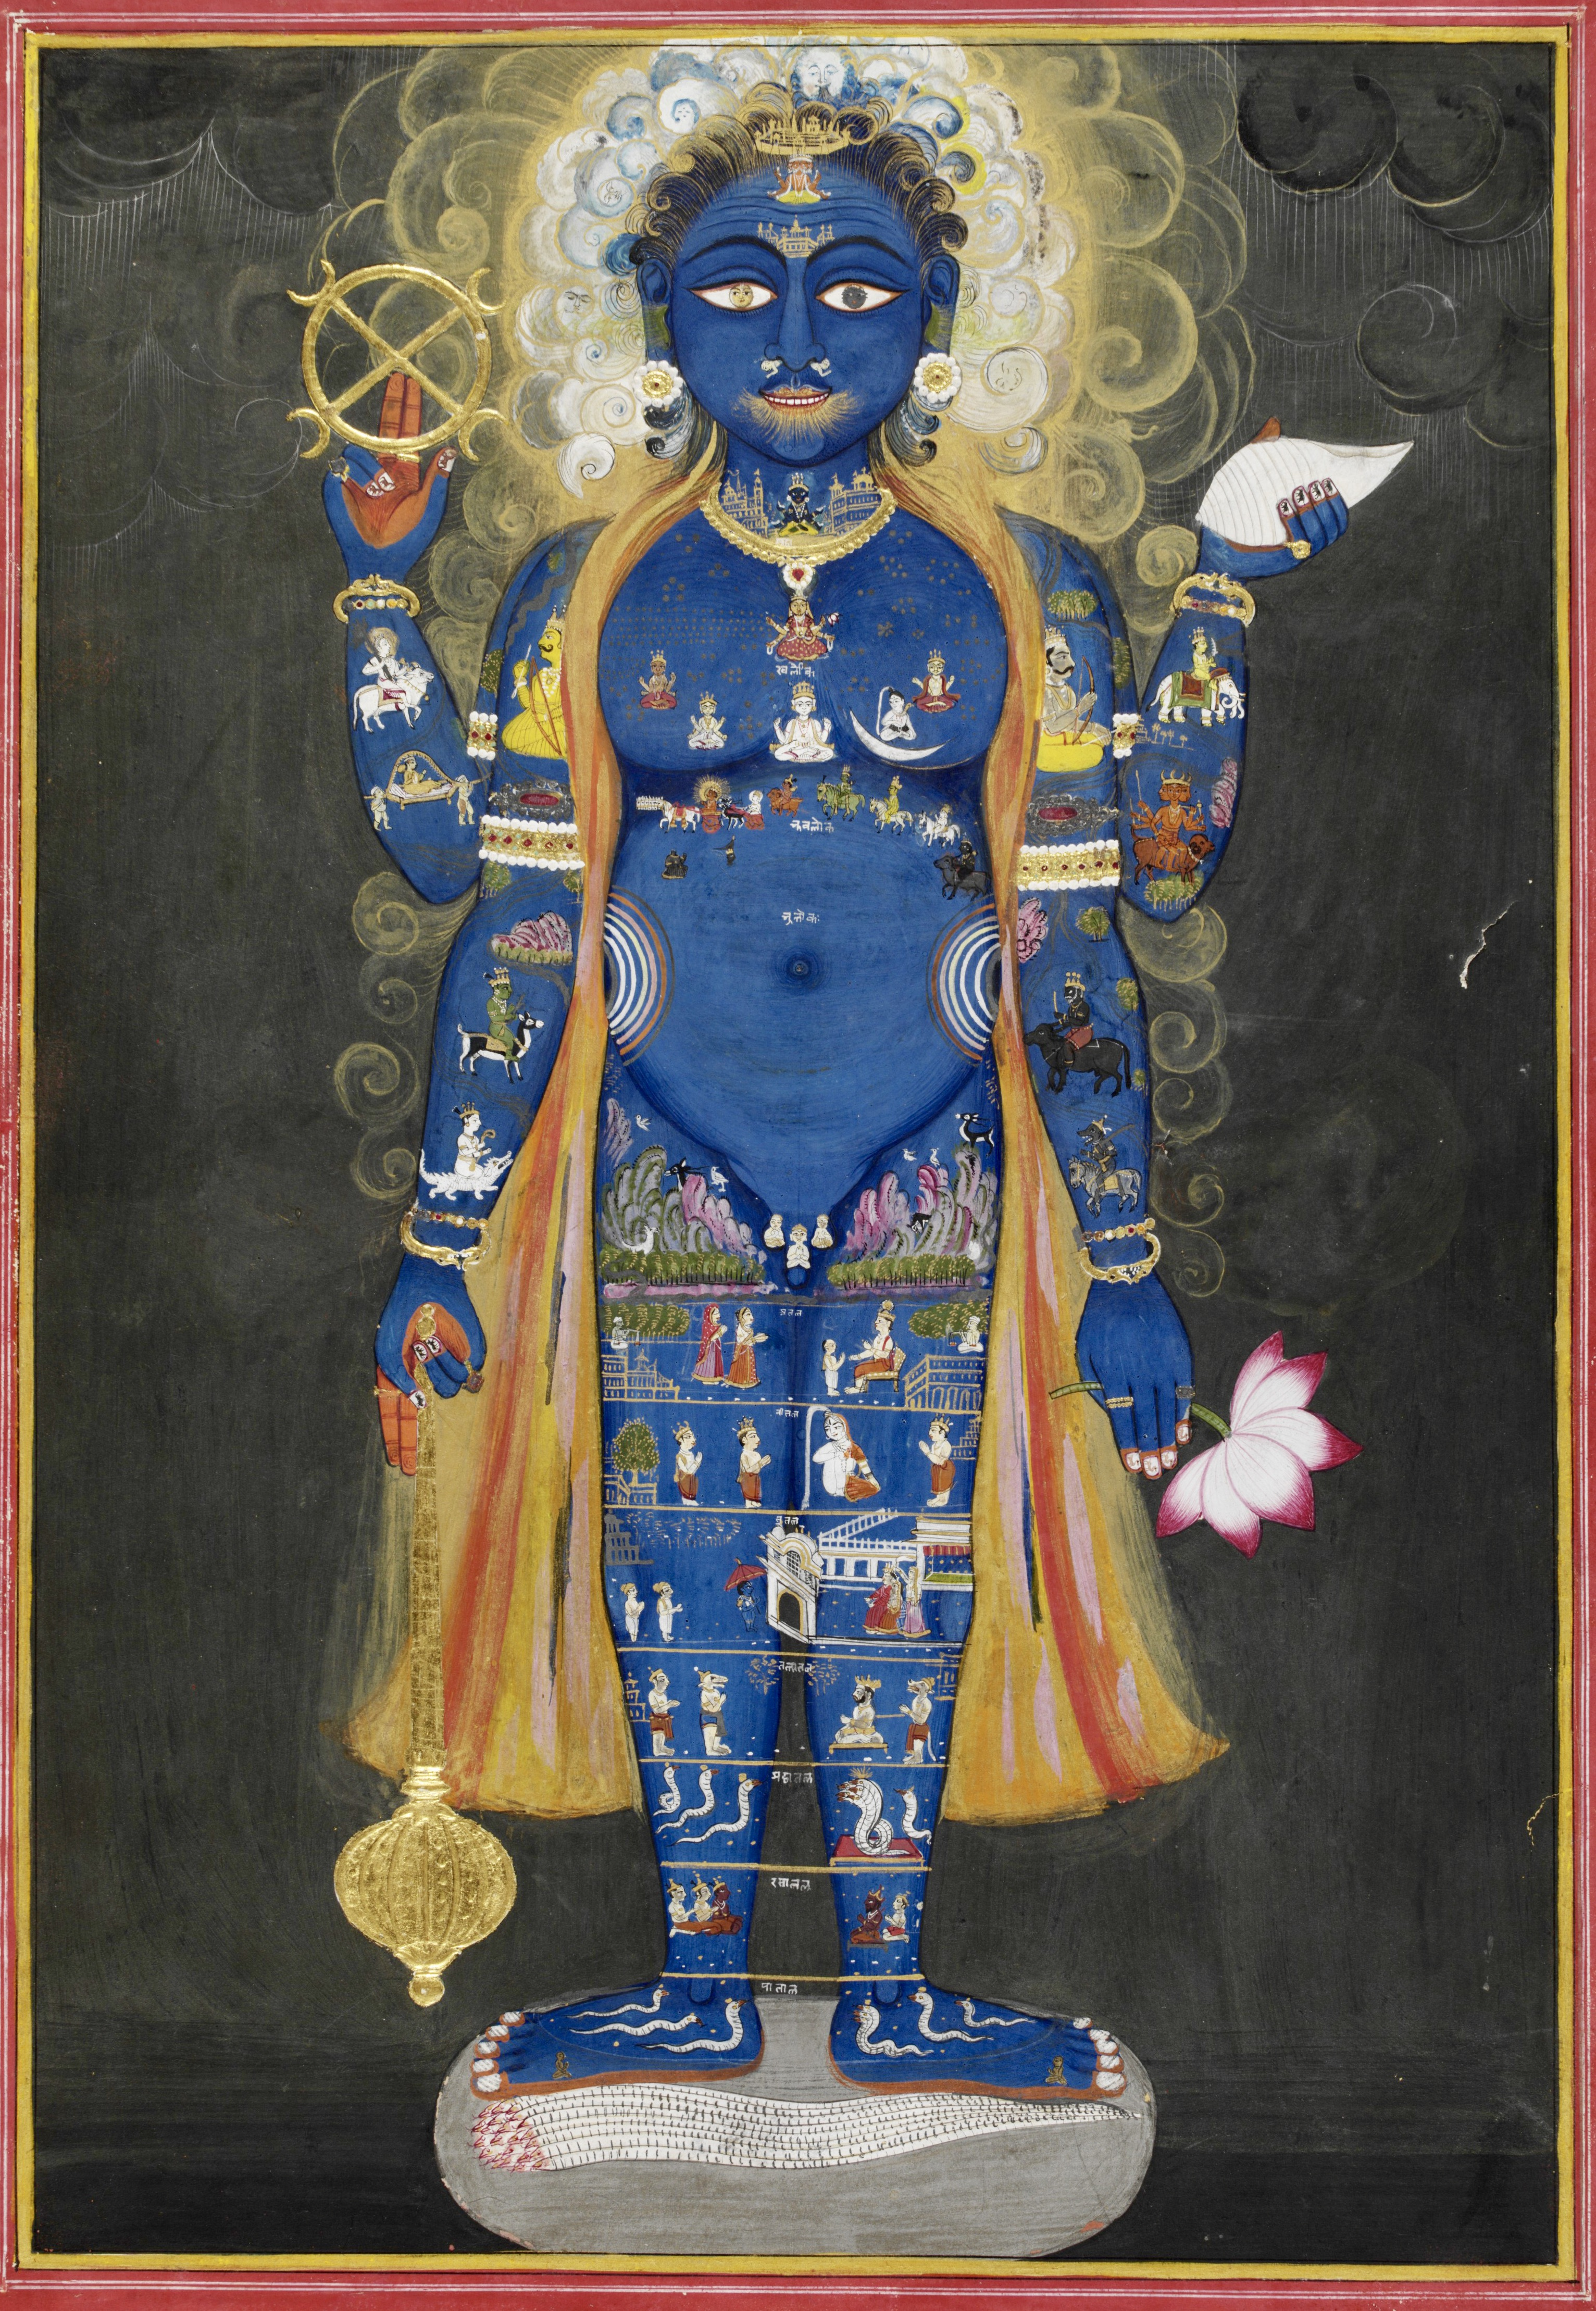
\includegraphics[width=1\textwidth]{pics/Vishnu_Vishvarupa_cropped.jpg}
	\caption{Viṣṇu Viśvarūpa, India, Rajasthan, Jaipur, ca. 1800–1820, Opaque watercolor and gold on paper, 38.5 × 28 cm, Victoria and Albert Museum, London, Given by Mrs. Gerald Clark.}
	\label{fig1}
      \end{figure}
\clearpage
  \begin{figure}[ht]
	\centering
  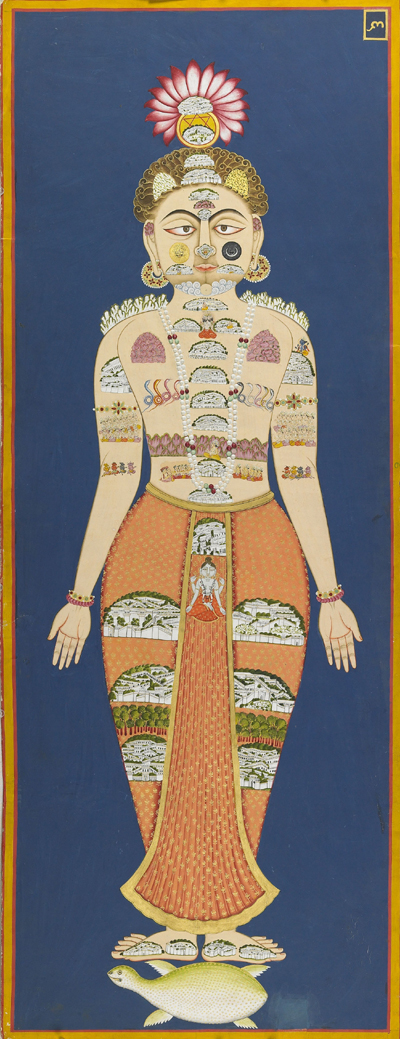
\includegraphics[width=0.5\textwidth]{pics/The_Equivalence_of_Self_and_Universe_(detail),_folio_6_from_the_Siddha_Siddhanta_Paddhati,_(Bulaki),_1824_(Samvat_1881);_122_x_46_cm._Mehrangarh_Museum_Trust..jpg}
	\caption{The Equivalence of Self and Universe (detail), folio 6 from the \textit{Siddhasiddhāntapaddhati} (Bulaki), India, Rajasthan, Jodhpur, 1824 (Samvat 1881), 122 x 46 cm, RJS 2378, Mehragarh Museum Trust.}
	\label{fig2}
      \end{figure}
      % \end{landscape}


\chapter{Bibliography}
 \label{sec:bibli}
   \clearpage
\newpage 
\thispagestyle{empty}
\quad  \addtocounter{page}{-1}

\printbibliography[heading=subbibintoc, title=Consulted Manuscripts, keyword=codex]

\printbibliography[heading=subbibintoc, title=Printed Editions, keyword=printsource]

\printbibliography[heading=subbibintoc, title=Secondary Literature, keyword=seclit]

\printbibliography[heading=subbibintoc, title=Online Sources, keyword=onlinesource]

\end{document}
